\documentclass[letterpaper,11pt]{article}

\usepackage{classDM}
\usepackage{hyperref}
\usepackage[normalem]{ulem}
\usepackage{inconsolata}
\usepackage{enumitem}
\usepackage{caption}

\usepackage[
backend=biber,
style=numeric,
]{biblatex} %Imports biblatex package
\addbibresource{sources.bib} %Import the bibliography file

\usepackage{bessex}

\title{Media Representation as a\\ 
\vspace{.1in} 
Predictor for Climate Policy Outcomes}
\author{Ben Essex, Emma Kerr}
\date{} 

\begin{document}
\maketitle

%\end{titlepage}

%%%%%%%%%%%%%%%%%%%%%%%%%%%%%%%%%%%%%%%%%%%%%%%%%%%%
%%%%%%%%%%%%%%%%%%%%%%%%%%%%%%%%%%%%%%%%%%%%%%%%%%%%
%%%%%%%%%%%%%%%%%%%%%%%%%%%%%%%%%%%%%%%%%%%%%%%%%%%%
\section{Introduction}

\vspace{.1in}

% Problem and motivation
\quad\textbf{Problem, Motivation, and Key Idea.}
Climate change is being increasingly viewed as an existential crisis. Legislators in the United States have, in recent years, stepped degree efforts to enact policies that might address this crisis. In a representative democracy, legislators are generally expected to act in accordance with the public good and in line with the views of their constituencies. This results in a complex interplay of news media, public opinion, and special interests, resulting in the enactment or failure of these policies. To many, the success of climate policy--its ``outcome"--is viewed as a question so important that its answer may dictate the very future of human life itself. As a result, there is great interest and value in better empirically understanding the complex dynamic by which these outcomes are produced.

This project seeks to address this question, and to analyze the nature of the dynamic between how media represents climate policies and the political outcomes for those policies. Primarily, we examine factors such as amount of media coverage, media source bias, sentiment on climate policy, and policy outcomes. A successful result for this study would be to make a contribution to the field of policy analysis, in the form of new techniques or analytic results. In this study, we introduce advanced methods in data acquisition, ETL, feature engineering, and analysis that are novel to this field. \\

\textbf{Previous Works.}
Studies to date on this topic have produced interesting results while taking a less quantitative approach. For example, one article focuses on normative questions \cite{boykoff2007climate}. Another examines the connection between viewership of a few popular cable news channels and viewer beliefs on climate change \cite{feldman2012climate}. However, previous works have generally examined this topic neither at massive scale nor with advanced data mining techniques.

%%%%%%%%%%%%%%%%%%%%%%%%%%%%%%%%%%%%%%%%%%%%%%%%%%%%
%%%%%%%%%%%%%%%%%%%%%%%%%%%%%%%%%%%%%%%%%%%%%%%%%%%%
%%%%%%%%%%%%%%%%%%%%%%%%%%%%%%%%%%%%%%%%%%%%%%%%%%%%
%%%%%%%%%%%%%%%%%%%%%%%%%%%%%%%%%%%%%%%%%%%%%%%%%%%%

\section{Data}

\vspace{.1in}

\subsection{Data Collection, Processing, and Feature Engineering}
In order to capture the complex interplay of factors contributing to policy outcomes, raw data was collected from several sources, and most underwent significant processing and transformation to be useful for analysis.\\

\quad\textbf{News Articles.} The corpus of news articles in this study was entirely sourced using the AYLIEN News API \cite{aylien}. In order to consume this API, we acquired an trial API key and built a harness around the API client. Once we developed a list of terms pertaining to policies under study (see \hyperref[dcap:ClimatePol]{Climate Policy}), we queried AYLIEN for any articles containing these terms, building a \verb|documents.json| file with over 40,000 articles since the beginning of the query window (27 months prior--the earliest AYLIEN would allow us to query). We stored each document with key metadata, including a document id, the published date, the article body, and the publishing source. Most of the time spent in this collection phase involved developing the harness and tweaking parameters to avoid exhausting AYLIEN's rate limit. The actual time to collect was less than a few hours using the harness.\\

\textbf{Climate Policy.}\label{dcap:ClimatePol} In order to produce a list of climate policies (bills and resolutions) to assess, we began with a manually generated list of terms related to climate (e.g. ``Climate Change," ``Carbon Dioxide," ``Methane," etc). We acquired an API key to the free ProPublica Congress API, for which we built another harness. Using this harness and the list of key terms, we queried the ProPublica API for bill topics or ``subjects" relevant to our key terms list \cite{propublica_congress_api}. When we had a list of subjects, we queried the ProPublica API for bills listed under those subjects. These bills comprise our list of ``climate policies." Like the news articles, the list of bills was restructured to fit a purpose-built JSON schema to ease storage and analysis. In addition to critical identifying information for each bill (including title, bill number, introduced date, etc.), we separately queried ProPublica for information on the latest House and/or Senate vote for each bill. For each vote, we computed and saved the overall proportion of votes for adoption of the bill, as well as the proportion for each party.

Due to the nature of the American legislative system, relatively few bills ever see a floor vote (e.g., only around 20 of the 138 bills we focused on). This meant clever feature engineering would be required to operationalize the outcome or ``success" of a bill. Since success could perhaps be measured in terms of the bill's distance from becoming public law, an ordinal representation for the bill's latest major action could be used as a measure of its success. For example, a bill that becomes public law might be assigned a \verb|last_action_ordinal| of 17, whereas a bill that has only just been introduced would be at 0. In order to determine the value of this new feature for each bill, we developed a harness to consume the U.S. Library of Congress API \cite{loc_api}. Using the bill data already acquired, we queried the API for the last major action code and last major action date. Since last major action code increments as bills progress through the legislative process (see \hyperref[appendix:B]{Appendix B}), we identified an opportunity to convert this value into an ordinal representation, which was saved along with the unix timestamp of the action in the bill data JSON file.\\

\textbf{Media Bias.} Another key factor in capturing the interplay of public opinion and policy outcome is certainly source bias. When dealing with policy, news sources are likely to present information in a way that aligns with the bias of the source. Furthermore, there is a human tendency to primarily consume sources with agreeable views, and this means the group primarily exposed to a biased representation often holds the same bias as the media outlet presenting it. The implications for public opinion and consequently policy outcomes are clear. So, in order to collect bias data for each news source, we utilized AllSides.com's source bias ratings, as manually annotated by their editors \cite{allsides_bias_ratings}. We then developed a tool to systematically access the source associated with every article acquired from AYLIEN and scrape AllSides.com for the bias rating of the source, saving an ordinal categorical bias rating $[1.0,\ 2.0,\ 3.0,\ 4.0,\ 5.0]$ with every document for which the source had an associated bias rating.\\

\textbf{Media Sentiment.} The last key piece of raw data needed is media sentiment. Core to an article's representation of a policy is the sentiment with which it presents it. Performing sentiment analysis at scale and in relation to climate policy would be a key enabling factor for a great deal of analysis of the dynamic between media representation and policy outcomes. Engineering a feature to capture sentiment was a multi-step process. We began with the bill terms list used for querying AYLIEN. This included bill number in multiple forms (e.g., H.R.1, H.Res. 1, etc.) and bill title. We tokenized each term using the spaCy English language tokenizer and created a mapping of start tokens to the corresponding token group. Then, we tokenized each article and iterated through each tokenization. If a token matched one of our starting tokens, the subsequent tokens were checked against the saved token group. If a match was found, a ``window" was saved--containing the matching text, the document id, the start and end indices in the document for the match, and an assigned instance id. By saving the start and end indices, later analysis could make use of a variable $\frac{k}{2}$ tokens on either side of the match.

After producing over 4,700 instances, we randomly sampled 56 instances to manually annotate. For each instance, we examined the $k$-gram in the text that subsumed the matching tokens ($k$ not including the number of tokens in the match itself). For this study, we set $k$ to 50 as a starting point that might produce sufficient context to accurately annotate instances. We labeled each instance as \verb|positive|, \verb|neutral|, or \verb|negative| about the climate policy in question. These instances became our training examples for $3 \times 19$ shot learning and subsequent sentiment classification using FLAN-T5 XL \cite{flan-t5-xl}.

%%%%%%%%%%%%%%%%%%%%%%%%%%%%%%%%%%%%%%%%%%%%%%%%%%%%
%%%%%%%%%%%%%%%%%%%%%%%%%%%%%%%%%%%%%%%%%%%%%%%%%%%%
%%%%%%%%%%%%%%%%%%%%%%%%%%%%%%%%%%%%%%%%%%%%%%%%%%%%
%%%%%%%%%%%%%%%%%%%%%%%%%%%%%%%%%%%%%%%%%%%%%%%%%%%%

\section{Analysis}

\vspace{.1in}
\subsection{Regression based on sentiment of article vs bill success}
    \textbf{Methodology} \\
    This analysis considers the 4,700 bill windows from the data collection step. These are the article windows collected from our Alyien scrape that could be re-matched to individual bill numbers. These matched windows, the sentiment assigned to them by FLAN-T5, and the bill's success all contribute for the data used in these regression models. 

    This study in particular only considers the subset of windows mentioning bills that were published before the last action of that specific bill. This is in hopes of capturing how the sentiment of media published before a bill affects the "success" of the particular bill. Success was measured by both the assigned ordinality of the data collection step, and the proportion of the House/Senate voting in favor of a particular bill. 

    Each one of these regressions also assigns bill sentiment to be the highest confidence of all 3 categories and sets the other categories to be 0. This is in hopes of streamlining the data and reducing noise that may be introduced by having multiple sentiment categories assigned to the same bill. In addition, the proportion of positive, negative, and neutral sentiment assigned to each bill window is aggregated and averaged and used as an independent variable in the regression models. \\
    \textbf{Results and findings}
    \begin{enumerate}
        \item Bill Sentiment vs Ordinality Regression
        \begin{center}
            \begin{figure}[htbp!]
                \centering
                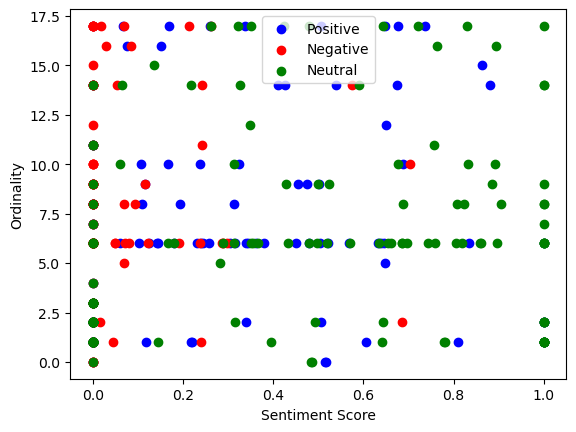
\includegraphics[width=10cm]{figs/fig_11.png}
                \captionsetup{ margin=2cm}
                    \caption{Scatter plot of all the windows in a bill and the aggregated positive, negative, and neutral sentiment vs the ordinality of the given bill.}
                \label{fig:scatterplot}
                \end{figure}
        \end{center}
    \vspace{-.74cm} % adjust the value as needed
    Linear regression of \href{fig:scatterplot}{Figure 1} gives a positive sentiment coefficient of 5.002, negative coefficient of 8.4371, and neutral of 3.7952 suggesting that as media increases in positive, negative, or neutral sentiment, a bill is more likely to be passed. This, of course, is a weak conclusion as the correlation coefficient is ~0.25 for positive and negative sentiment and ~0.19 for neutral sentiment, although the results found are interesting and warrant further investigation. \\

    Here is a similar plot on the proportion of positive, neutral, and negative instances per bill. A similar conclusion can be made with a neglegable correlation coefficient. 

    \begin{center}
            \begin{figure}[htbp!]
                \centering
                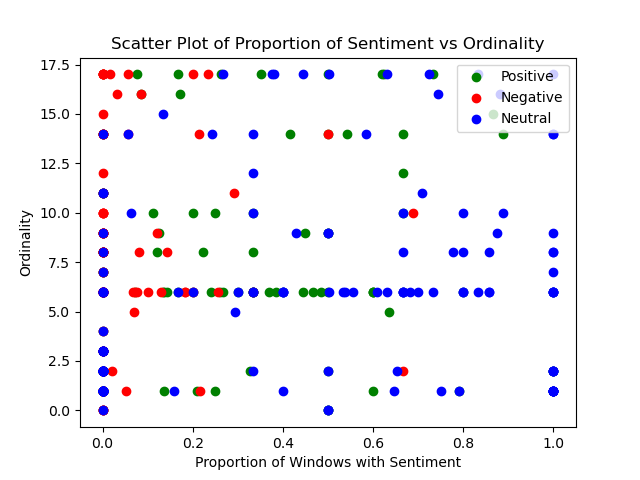
\includegraphics[width=12cm]{figs/foo.png}
                \captionsetup{ margin=2cm}
                    % \caption{Scatter plot of all the windows in a bill and the aggregated positive, negative, and neutral sentiment vs the ordinality of the given bill.}
                \label{fig:scatterplot}
                \end{figure}
        \end{center}

    \item Positive and Negative Sentiment vs Congress Vote Proportion
    \end{enumerate}


%%%%%%%%%%%%%%%%%%%%%%%%%%%%%%%%%%%%%%%%%%%%%%%%%%%%
%%%%%%%%%%%%%%%%%%%%%%%%%%%%%%%%%%%%%%%%%%%%%%%%%%%%
%%%%%%%%%%%%%%%%%%%%%%%%%%%%%%%%%%%%%%%%%%%%%%%%%%%%
%%%%%%%%%%%%%%%%%%%%%%%%%%%%%%%%%%%%%%%%%%%%%%%%%%%%

\section{Ethics}

\vspace{.1in}

\begin{enumerate}
    \item Ethical considerations and implications of the study. (For example, systematic bias not in the news articles but in the provider, AYLIEN; bias ingrained in FLAN-T5-xl)
\end{enumerate}

%%%%%%%%%%%%%%%%%%%%%%%%%%%%%%%%%%%%%%%%%%%%%%%%%%%%
%%%%%%%%%%%%%%%%%%%%%%%%%%%%%%%%%%%%%%%%%%%%%%%%%%%%
%%%%%%%%%%%%%%%%%%%%%%%%%%%%%%%%%%%%%%%%%%%%%%%%%%%%
%%%%%%%%%%%%%%%%%%%%%%%%%%%%%%%%%%%%%%%%%%%%%%%%%%%%

\section{Drawbacks, Deficiencies, and Obstacles}

\vspace{.1in}

\begin{enumerate}
    \item Limitations of the dataset and models
    \item Challenges encountered during the project
\end{enumerate}

%%%%%%%%%%%%%%%%%%%%%%%%%%%%%%%%%%%%%%%%%%%%%%%%%%%%
%%%%%%%%%%%%%%%%%%%%%%%%%%%%%%%%%%%%%%%%%%%%%%%%%%%%
%%%%%%%%%%%%%%%%%%%%%%%%%%%%%%%%%%%%%%%%%%%%%%%%%%%%
%%%%%%%%%%%%%%%%%%%%%%%%%%%%%%%%%%%%%%%%%%%%%%%%%%%%

\section{Conclusion}

\vspace{.1in}

\begin{enumerate}
    \item Summary of key findings and contributions
    \item Suggestions for future research
\end{enumerate}

%%%%%%%%%%%%%%%%%%%%%%%%%%%%%%%%%%%%%%%%%%%%%%%%%%%%
%%%%%%%%%%%%%%%%%%%%%%%%%%%%%%%%%%%%%%%%%%%%%%%%%%%%
%%%%%%%%%%%%%%%%%%%%%%%%%%%%%%%%%%%%%%%%%%%%%%%%%%%%
%%%%%%%%%%%%%%%%%%%%%%%%%%%%%%%%%%%%%%%%%%%%%%%%%%%%

\clearpage

\section*{Appendix A: Distribution of Work}

% table goes here

%%%%%%%%%%%%%%%%%%%%%%%%%%%%%%%%%%%%%%%%%%%%%%%%%%%%
%%%%%%%%%%%%%%%%%%%%%%%%%%%%%%%%%%%%%%%%%%%%%%%%%%%%
%%%%%%%%%%%%%%%%%%%%%%%%%%%%%%%%%%%%%%%%%%%%%%%%%%%%
%%%%%%%%%%%%%%%%%%%%%%%%%%%%%%%%%%%%%%%%%%%%%%%%%%%%

\clearpage

\section*{Appendix B: Table of Legislative Action Codes}\label{appendix:B}

\begin{table}[!h]
\centering
\footnotesize
\begin{tabular}{llll}
\hline
\textbf{Action} & \textbf{Code} & \textbf{Action} & \textbf{Code} \\
\hline
Introduced in House & 1000 & House committee discharged & 5500 \\
Referred to House committee & 2000 & House floor actions & 7000 \\
Referred to House subcommittee & 3000 & Passed/agreed to in House & 8000 \\
House committee/subcommittee actions & 4000 & Failed of passage/not agreed to in House & 9000 \\
House committee/subcommittee hearings & 4100 & Introduced in Senate & 10000 \\
House committee/subcommittee markups & 4200 & Referred to Senate committee & 11000 \\
House committee time extension & 4900 & Referred to Senate subcommittee & 12000 \\
House discharge petition filed & 4950 & Senate committee/subcommittee actions & 13000 \\
Reported to House & 5000 & Senate committee/subcommittee hearings & 13100 \\
Senate committee/subcommittee markups & 13200 & Conference report disagreed to in House & 22000 \\
Senate committee time extension & 13900 & Conference report agreed to in Senate & 23000 \\
Reported to Senate & 14000 & Conference report disagreed to in Senate & 24000 \\
Senate committee discharged & 14500 & Roll call votes on measures in House & 25000 \\
Senate committee report filed after reporting & 14900 & Roll call votes on measures in Senate & 26000 \\
Senate floor actions & 16000 & Presented to President & 28000 \\
Passed/agreed to in Senate & 17000 & Signed by President & 29000 \\
Failed of passage/not agreed to in Senate & 18000 & Sent to Archivist unsigned by President & 29100 \\
Resolving differences -- House actions & 19000 & Pocket vetoed by President & 30000 \\
Resolving differences -- Senate actions & 20000 & Vetoed by President & 31000 \\
Conference committee actions & 20800 & Passed House over veto & 32000 \\
Conference report filed & 20900 & Failed of passage in House over veto & 33000 \\
Conference report agreed to in House & 21000 & Passed Senate over veto & 34000 \\
Failed of passage in Senate over veto & 35000 & Private Law signed by President & 42000 \\
Became Public Law & 36000 & Private Law unsigned by President & 43000 \\
Public Law signed by President & 37000 & Private Law enacted over veto & 44000 \\
Public Law unsigned by President & 38000 & Private Law by other means & 45000 \\
Public Law enacted over veto & 39000 & Line item veto by President & 46000 \\
Public Law by other means & 40000 & Disapproval bill in House & 47000 \\
Became Private Law & 41000 & Disapproval bill in Senate & 48000 \\
House amendment offered & 71000 & Senate amendment submitted & 91000 \\
House amendment agreed to & 72000 & Senate amendment referred to committee & 92000 \\
House amendment considered as adopted & 72500 & Senate amendment proposed (on the floor) & 93000 \\
House amendment not agreed to & 73000 & Senate amendment agreed to & 94000 \\
Other House amendment actions & 74000 & Senate amendment not agreed to & 95000 \\
Roll call votes on amendments in House & 75000 & Other Senate amendment actions & 96000 \\
Roll call votes on amendments in Senate & 97000 & & \\
\hline
\end{tabular}
\end{table}



%%%%%%%%%%%%%%%%%%%%%%%%%%%%%%%%%%%%%%%%%%%%%%%%%%%%
%%%%%%%%%%%%%%%%%%%%%%%%%%%%%%%%%%%%%%%%%%%%%%%%%%%%
%%%%%%%%%%%%%%%%%%%%%%%%%%%%%%%%%%%%%%%%%%%%%%%%%%%%
%%%%%%%%%%%%%%%%%%%%%%%%%%%%%%%%%%%%%%%%%%%%%%%%%%%%

\clearpage


\printbibliography
%%% *** IMPORTANT *** ... use for bib mgmt: https://www.overleaf.com/learn/latex/Bibliography_management_in_LaTeX 
%%% (see sources.bib)

\end{document}
